\documentclass[a4paper,article]{article}

%====Шрифты========
\usepackage{fontspec}
\usepackage[14pt]{extsizes}
\setmainfont{Times New Roman}
\setmonofont{Courier New}[Scale=1.0]


\usepackage{ragged2e} % для выравнивания по ширине
\usepackage{ulem}   % для подчеркивания
\usepackage{enumitem}% для списков

%todo gather и вставить
%Языки
\usepackage[english, russian]{babel}

%========Параметры страницы=======
\usepackage[left=3cm, top=2cm, right=1.5cm, bottom=2cm]{geometry}
\usepackage[onehalfspacing]{setspace}

%=========Параметры текста===========
%Абзацный отступ
\setlength{\parindent}{1.25cm}

%=============Таблицы==========
\usepackage{xltabular}% Таблица
\usepackage{csvsimple}%считывание из csv
\usepackage{caption}%для изменения названий таблиц и рисунков
\DeclareCaptionLabelFormat{gosttable}{Таблица~#2~-- }
\captionsetup[table]{labelformat=gosttable, labelsep=none, justification=raggedright, singlelinecheck=false}%, aboveskip=0pt, belowskip=0pt}


%============содержание=============
\usepackage{tocloft}
%отступ после заголовка "Содержание"
\setlength{\cftaftertoctitleskip}{1.5pt}
%Нормальный текст "Содержание"
\addto\captionsrussian{\renewcommand{\contentsname}{\normalsize\bfseries\hfil\selectfont СОДЕРЖАНИЕ}}
%стили точек в Содержании
\renewcommand{\cftdot}{\normalfont.}%Стиль точек
\renewcommand{\cftdotsep}{1}%расстояние между точками
\renewcommand{\cftsecdotsep}{\cftdotsep}%добавить точки в содержании для \section
\renewcommand{\cftsubsecdotsep}{\cftdotsep}%добавить точки в содержании для \subsection
\renewcommand{\cftsubsubsecdotsep}{\cftdotsep}%добавить точки в содержании для \subsubsection
\renewcommand{\cftsecfont}{\normalfont}%Обычный шрифт в содержании
\renewcommand{\cftsecpagefont}{\normalfont}%Страницы тоже обычным
%настраиваем отступы в содержании у глав в 1.5 пункта
\renewcommand{\cftbeforesecskip}{1.5pt}
\renewcommand{\cftsecaftersnum}{.}%добавляем точку у номера section в содержании
\renewcommand{\cftsubsecaftersnum}{.}%добавляем точку у номера subsection в содержании
\renewcommand{\cftsubsubsecaftersnum}{.}%добавляем точку у номера subsubsection в содержании

%============Настраиваем заголовки===========
\usepackage{titlesec}
\titlespacing*{\section}
{\parindent}{0em}{0em}%добавляем абзацный отступ перед \section 
\titlespacing*{\subsection}
{\parindent}{0em}{0em}%добавляем абзацный отступ перед \subsection 
\titlespacing*{\subsubsection}
{\parindent}{0em}{0em}%добавляем абзацный отступ перед \subsubsection 

\titleformat{\section}%переопределяем стили section
  {\normalfont\bfseries}%делаем жирным, 14 шрифт
  {\thesection. }
  {0cm}
  {}
\titleformat{\subsection}%переопределяем стили subsection
  {\normalfont\bfseries}%делаем жирным
  {\thesubsection. }
  {0cm}
  {}
\titleformat{\subsubsection}%переопределяем стили subsubsection
  {\normalfont\bfseries}%делаем жирным
  {\thesubsubsection. }
  {0cm}
  {}

\usepackage{indentfirst}% добавляет отступ для первого абзаца после section

%==========ссылки===========
\usepackage{color}
\definecolor{Black}{RGB}{0,0,0}
%без colorlinks вокруг ссылок появляются рамки
%если не зачернить ссылки, то в оглавлении и в других местах будут яркие цвета
\usepackage[colorlinks, allcolors=Black]{hyperref}
%шрифт для URL
\urlstyle{rm}
\usepackage{xurl}%разрешает переносы в URL

%========картинки========
\usepackage{graphicx}
\graphicspath{{images/}}%указываем папку где будут лежать картинки
\usepackage[labelsep=none]{caption}%убираем разделитель между "Рис. X" и названием рисунка
%изменяем разделитель
\DeclareCaptionLabelFormat{gostfigure}{Рисунок~#2~-- }
\captionsetup[figure]{labelformat=gostfigure, labelsep=none, justification=centering, belowskip=-10pt} %aboveskip=12pt, belowskip=-4pt}
%Чтобы рисунок не убегал вниз
\usepackage{float}
%Для оптикаемых картинок
\usepackage{wrapfig}

%======картинки и таблицы======
\setlength{\intextsep}{0.5\baselineskip}%отступ между float'ом внутри текста и текстом
\setlength{\textfloatsep}{0.5\baselineskip}%отступ между текстом и float сверху/снизу страницы
\setlength{\floatsep}{0.5\baselineskip}% отступ между двумя float'ами подряд
%отступы вокруг подписей
\setlength{\abovecaptionskip}{0.5\baselineskip}%от картинки/таблицы до подписи
%\setlength{\belowcaptionskip}{-7.5pt} % от подписи до следующего текста


%==========для формул==============
\usepackage{amsmath}
%% Перенос знаков в формулах (по Львовскому)
\newcommand*{\hm}[1]{#1\nobreak\discretionary{}
{\hbox{$\mathsurround=0pt #1$}}{}}
\usepackage{amsfonts}%некоторые мат. символы
%отступы сверху и снизу
\makeatletter
\g@addto@macro\normalsize{%
  \setlength{\abovedisplayskip}{0pt}
  \setlength{\belowdisplayskip}{0pt}
  \setlength{\abovedisplayshortskip}{-8pt}
  \setlength{\belowdisplayshortskip}{6pt}
}
\makeatother


%=========для доказательств, примеров, теорем и т.д.=============
\usepackage{amsthm}
\newtheoremstyle{mystyle}
  {0pt}%пространство сверху
  {0pt}%пространство снизу
  {\normalfont}%шрифт тела
  {0pt}%отступ
  {\normalfont\indent}%шрифт заголовка
  {.}%пунктуация после заголовка
  { }%пространство после заголовка
  {}%дополнительные настройки
\theoremstyle{mystyle}
\newtheorem{theorem}{Теорема}[section]
\newtheorem{statement}{Утверждение}
\newtheorem*{example}{Пример}
\makeatletter%настраиваем доказательство(убираем курсив, добавляем отступ)
\renewenvironment{proof}[1][\proofname]{%
  \par\pushQED{\qed}%
  \normalfont%обычный шрифт для заголовка и тела
  \topsep-2pt\@plus-2pt\relax
  \trivlist
  \item[\indent\hskip\labelsep #1\@addpunct{.}]\ignorespaces
}{%
  \popQED\endtrivlist\@endpefalse
}
\makeatother


%настраиваем стили для кода в приложении
\usepackage{listings}
\lstset{
  basicstyle=\ttfamily\fontsize{12pt}{14pt}\selectfont,
  breaklines=true,
  showstringspaces=false,
  keepspaces=true
}


%=======Собственные команды==========
%Центровка и стиль заголовков для введение списка лит-ры и т.д.
\newcommand{\customsection}[1]{
	\phantomsection%создаем точку для перехода через содержание
  	\addcontentsline{toc}{section}{#1}%добавляем пункт в содержание
    {
        \centering
        \textbf{\normalsize\selectfont #1} \par
    }
}

%собственный список чтобы не писать стили каждый раз везде
\newcommand{\mystyleitemize}[1]{
  \begin{itemize}[label=--, 
				leftmargin=0pt,%общий отступ списка слева
    				labelindent=\parindent,%отступ метки от левого края элемента
    				labelsep=1cm,%Отступ между меткой и текстом
    				itemindent=*,%автоматический отступ элемента
    				nolistsep%убрать промежутки между элементами
    				]
    #1
  \end{itemize}
}

\newenvironment{mytable}[3][h]{
  \def\mytablecaption{#2}%временные переменные
  \def\mytablelabel{#3}%временные параменные
  \begin{table}[#1]
    \vspace{-2pt}
    \centering
    \caption{\mytablecaption}
    \vspace{-14pt}
    \label{\mytablelabel}
}{
    \vspace{-16pt}
  \end{table}
}


%5. Ссылки на:
%   - Исходный код (GitHub/GitLab)
%   - Развернутое веб-приложение (Hugging Face Space / Render / Railway) - практика
%   - Опубликованные модели (Hugging Face Hub) - практика
%6. Выводы по работе - заключение
%7. **Рефлексия:** Что получилось лучше всего? С какими трудностями столкнулись? Что бы сделали иначе? - заключение


\begin{document}
\begin{sloppypar}
	\begin{titlepage}
		\begin{center}
			Министерство науки и высшего образования Российской Федерации \\
     		Федеральное государственное автономное образовательное учреждение высшего образования \\
        		<<КАЗАНСКИЙ (ПРИВОЛЖСКИЙ) ФЕДЕРАЛЬНЫЙ УНИВЕРСИТЕТ>> \\
        		Институт Вычислительной математики и информационных технологий
		\end{center}
		
		\vfill
		
		\begin{center}
			Отчет \\
			по обработке естественных языков. \\
			Лаборатарный практикум 1
		\end{center}
		
		\vfill		
		
		\noindent
		\begin{xltabular}{\textwidth} {
                >{\hsize=0.8\hsize} X
                >{\hsize=0.2\hsize} X }
            Обучающийся \uline{Генералов Вадим Викторович \quad гр.09-435} & \underline{\hspace{2cm}} \\
            
            \makebox[0.16\linewidth][r]{} \makebox[0.48\linewidth][c]{\fontsize{8pt}{0pt}\selectfont (ФИО студента)} \makebox[0.14\linewidth][c]{\fontsize{8pt}{0pt}\selectfont (Группа)} & \makebox[0.12\linewidth][c]{\fontsize{8pt}{0pt}\selectfont (Подпись)} \\
            & \\
            & \\
            & \\
            & \\
            Преподаватель: & \\
            & \\
            Арабов М.К.  & \underline{\hspace{2cm}}\\
            & \makebox[2cm][c]{\fontsize{8pt}{0pt}\selectfont (Подпись)}\\
            Дата сдачи отчета <<\uline{\hspace{1cm}}>>\uline{\hspace{3cm}}2025 г. & \\
        \end{xltabular}
		
		\vfill
		
		\begin{center}
            Казань -- 2025
        \end{center}
	\end{titlepage}
	
	\newpage

    \setcounter{page}{2}

    \tableofcontents

    \newpage
    
    \customsection{ВВЕДЕНИЕ}
    
		Лабораторная работа выполнена в рамках предмета <<Обработка естественных языков>> по программе 2 курса магистратуры.
	
		Целью практики является формирование целостного практического понимания полного цикла обработки текстовых данных в области обработки естественного языка (Natural Language Processing) -- от сбора и подготовки неструктурированных текстов до построения и развертывания инференс-моделей. Особое внимание уделить осмысленному сравнению и критическому анализу подходов к одной из ключевых задач NLP — токенизации.
	
		Для достижения данной цели необходимо выполнить следующие задачи:
	
		\mystyleitemize{
    			\item освоить методы сбора и предобработки текстовых корпусов, включая извлечение данных из веб-источников;
    			\item реализовать и провести экспериментальное сравнение традиционных и современных методов токенизации, стемминга и лемматизации;
    			\item получить практические навыки обучения подсловных моделей токенизации (BPE, WordPiece, Unigram);
    			\item научиться проводить количественный и качественный анализ эффективности различных алгоритмов с применением объективных метрик;
    			\item разработать и оформить результаты исследования в виде интерактивного веб-интерфейса и API-сервиса;
    			\item освоить процесс публикации обученных моделей и сопроводительной документации в открытых репозиториях.
		}

	\newpage
	\section{Инструментарий}
	
		Для выполнения лабораторной работы использовался современный стек инструментов и библиотек Python, обеспечивающий полный цикл обработки текстовых данных, машинного обучения и визуализации результатов.
		
		Для сбора и обработки текстовых данных использовались:
		
		\mystyleitemize{
    			\item requests. Библиотека использовалась для выполнения HTTP-запросов к веб-сайтам новостных агентств. Она обеспечивает получение HTML-кода страниц;
    			\item BeautifulSoup. Основной инструмент для парсинга HTML-документов и извлечения нужных фрагментов текста. Применяется для поиска мета-тегов, выделения содержимого статьи, поиска категорий публикаций, получения всех гиперссылок со страниц;
    			\item urllib.parse (urljoin, urlparse). Применяется для нормализации и объединения относительных и абсолютных URL;
    			\item time. Используется для соблюдения задержек между запросами к одному домену;
    			\item json. Библиотека для сериализации собранных данных в формате JSON Lines (JSONL), где каждая строка -- отдельная статья;
    			\item re. Используется для фильтрации неподходящих ссылок, поиска шаблонов дат в тексте HTML, выявления блоков с текстом статьи по ключевым словам в классах;
    			\item dateparser и dateutil.parser. Обе библиотеки применяются для распознавания и нормализации дат публикации из различных форматов. dateparser автоматически определяет дату из строк на естественном языке или из HTML-тегов. dateutil.parser используется как резервный вариант для ISO-форматов.
		}
		
		Для предварительной обработки и очистки текста использовалась библиотека nltk, которая применяется для работы с лингвистическими данными и в данном модуле отвечает за удаление стоп-слов.
		
		Для проектирования универсального модуля предобработки текстов использовалась библиотека html. Она используется для декодирования и замены некоторых html сущностей.
		
		Для сравнительного анализа методов токенизации и нормализации использовались:
		
		\mystyleitemize{
    			\item csv. Используется для сохранения результатов эксперимента в табличном виде;
    			\item razdel. Один из лучших токенизаторов для русского языка, оптимизированный под морфологические особенности;
    			\item spacy. Для токенизации, лемматизации;
    			\item sentence-transformers. Используется для оценки семантической согласованности текста на основе схожести ембедингов;
    			\item sklearn.metrics.pairwise. Для подсчёта семантической близости между эмбедингами.
		}
		
		На этапе обучения subword моделей токенизации использовались следующие библиотеки:
		
		\mystyleitemize{
    			\item tokenizers (Hugging Face). Это основная библиотека для работы с подсловными моделями токенизации;
    			\item pathlib. Работа с путями к файлам и каталогам в объектно-ориентированном виде;
    			\item rapidfuzz. Используется для вычисления нормализованного расстояния Левенштейна между исходным и восстановленным текстом (после токенизации и декодирования).
Позволяет оценить качество реконструкции -- насколько точно модель токенизатора может восстановить исходную строку;
    			\item sklearn.metrics.pairwise. Для подсчёта семантической близости между эмбедингами.
		}
		
		При разработке веб приложения использовались следующие библиотеки:
		
		\mystyleitemize{
    			\item Streamlit. Создание веб-интерфейса, через который пользователь взаимодействует с системой;
    			\item Plotly Express. Используется для отображения гистограмм и барчартов в интерфейсе и HTML-отчетах;
		}
		
	\section{Разработка проекта}
	
		\subsection{Парсинг новостных сайтов и приведение текстов к JSONL файлу}
		
			Этот модуль автоматически собирает новостные статьи с русскоязычных сайтов.
			
			Он проходит по индексным страницам, собирает ссылки на публикации, парсит каждую статью, очищает её и сохраняет в единый корпус в формате .jsonl, где каждая строка -- это отдельная статья. Затем мы можем использовать эти данные для дальнейших NLP эксперементов.
			
			Модуль организован модульно и предельно безопасно по отношению к внешним сайтам, имеет задержку и фильтрации.
			
			На рисунке \ref{fig:corpusjsonl} изображена часть файла jsonl, содержащего распарсенные статьи.
			
			\begin{figure}[h]
        			\centering
        			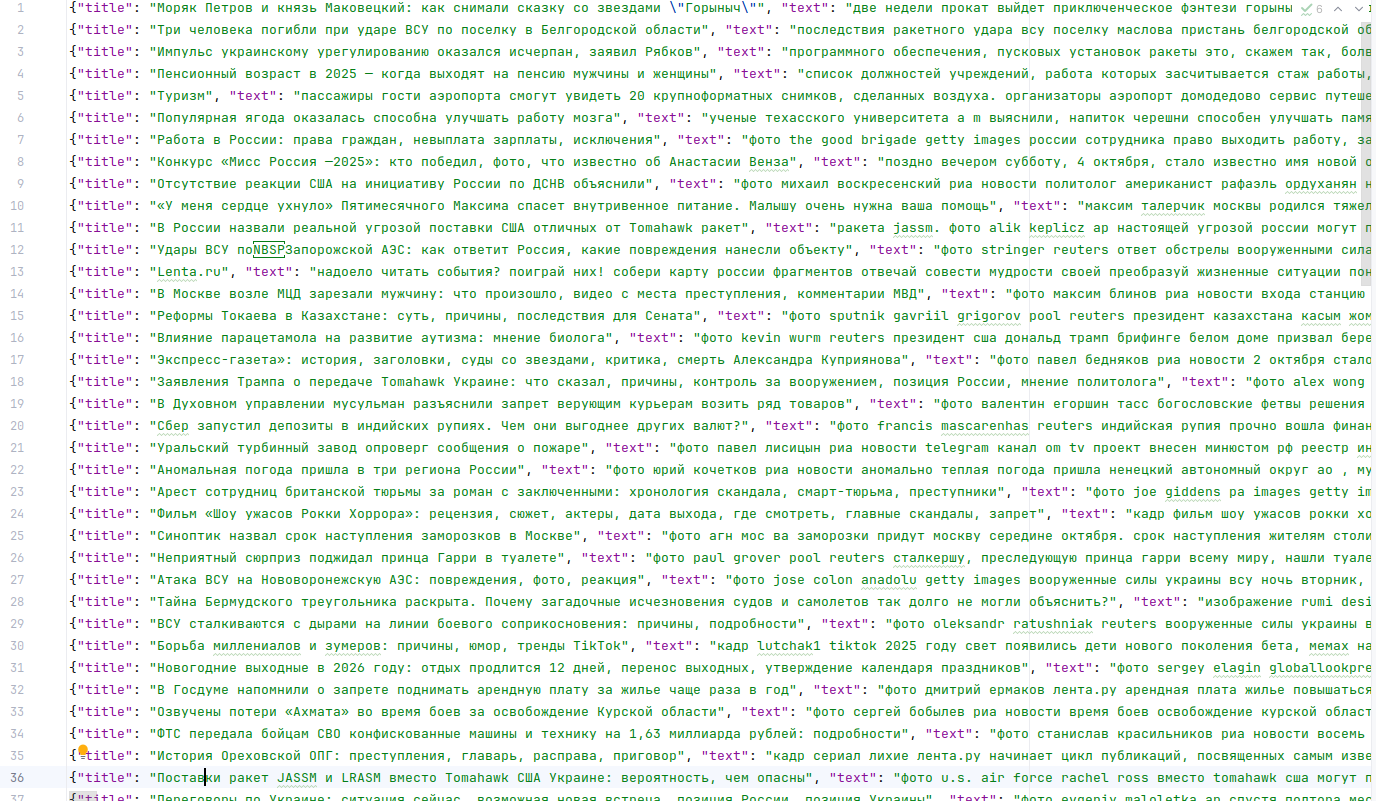
\includegraphics[width=0.9\linewidth]{corpusjsonl.png}
        			\caption{Пример файла corpus.jsonl}
        			\label{fig:corpusjsonl}
    			\end{figure}
	
		\subsection{Обработка и очистка текстов}
			
			Этот модуль -- универсальный препроцессор текстовых данных, который очищает сырой HTML-контент новостных статей и превращает его в стандартизованный, пригодный для NLP-анализов текст.

			Он устраняет шум (HTML-разметку, спецсимволы, URL, дубликаты пробелов и мусорные конструкции), нормализует формат текста (пробелы, регистр) и при необходимости удаляет стоп-слова.

			Именно этот модуль используется на предыдущем этапе при формировании корпуса текста, чтобы итоговый jsonl содержал текст, очищенный от HTML и имел некоторую предобработку.
			
		\subsection{Модуль предобработки}
		
			Цель данного модуля -- это создать гибкий, конфигурируемый препроцессор, способный приводить тексты к единому формату перед токенизацией и последующим анализом.
Основная идея -- стандартизировать текст, устранив вариативность пунктуации, форматирования, чисел, ссылок и сокращений. Это критично для обеспечения стабильности работы токенизаторов и моделей NLP.

			В результате работы данного модуля мы получаем следующий артефакт -- другой jsonl файл, в который мы сохраняем результат работы данного модуля.
			
			Пример части этого файла изображен на рисунке \ref{fig:processedjsonl}.
			
			\begin{figure}[h]
        			\centering
        			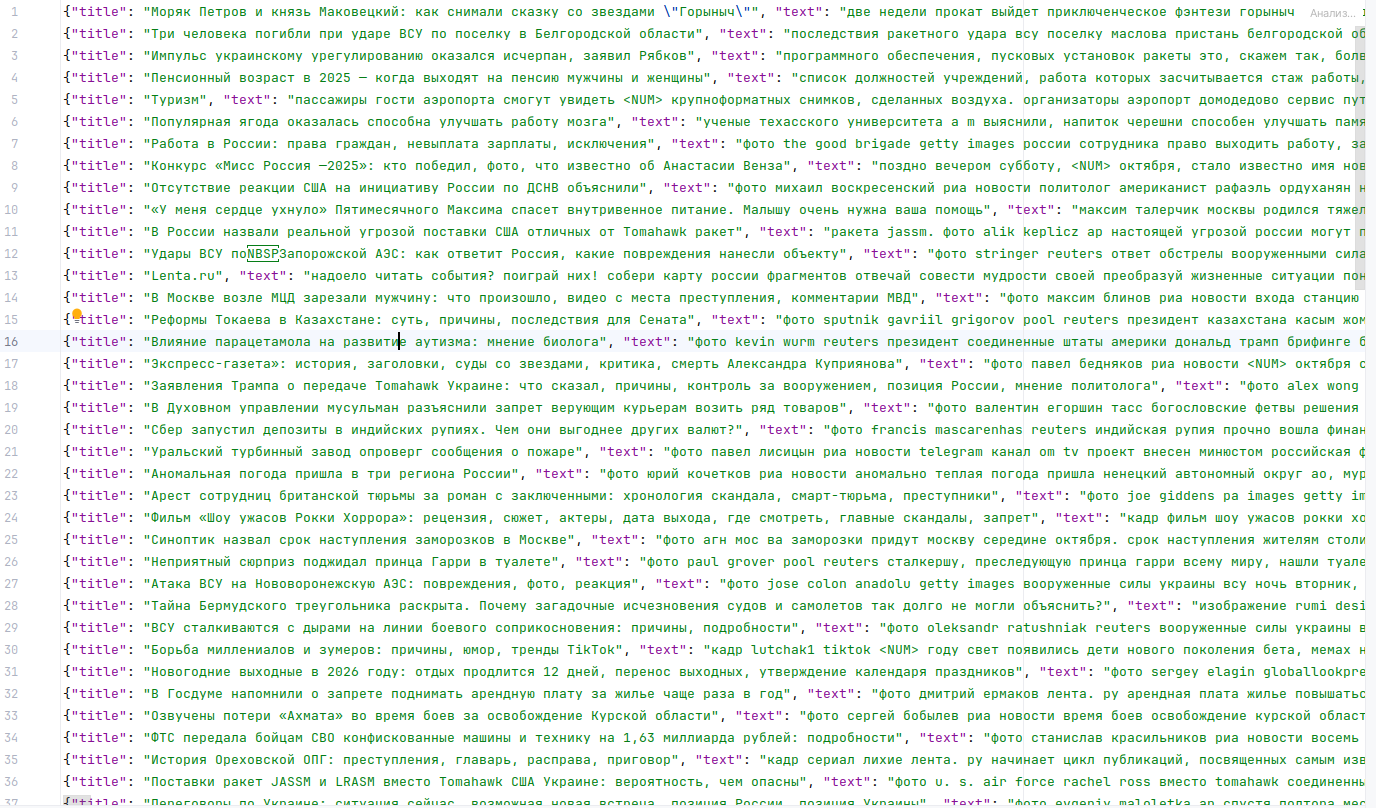
\includegraphics[width=0.9\linewidth]{processedjsonl.png}
        			\caption{Пример файла processed.jsonl}
        			\label{fig:processedjsonl}
    			\end{figure}
		
		\subsection{Сравнительный анализ методов токенизации и нормализации}
			
			Целью данного этапа является проведение комплексного эмпирического анализа эффективности различных методов токенизации и нормализации текста на русском языке.
			
			Этот шаг завершает блок подготовки данных, позволяя количественно и качественно сравнить, насколько разные комбинации токенизаторов и нормализаторов влияют на размеры словаря, OOV, скорость обработки, сохранение семантического смысла.
			
			В качестве результата работы мы получаем csv файл, в котором наглядно можем увидеть сравнение алгоритмов на разных метриках. Пример вывода данных для моего случая представлен на рисунке \ref{fig:tokenizationmetrics}.
			
			\begin{figure}[h]
        			\centering
        			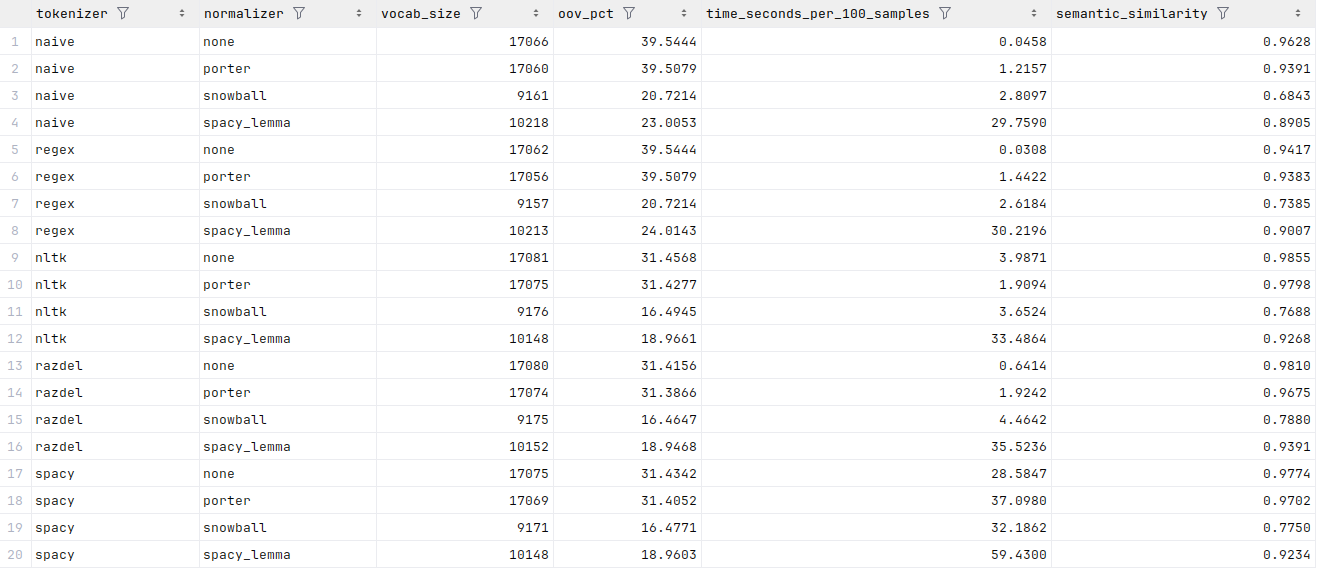
\includegraphics[width=0.9\linewidth]{tokenizationmetrics.png}
        			\caption{Пример файла tokenizationmetrics.csv}
        			\label{fig:tokenizationmetrics}
    			\end{figure}
			
		\subsection{Обучение подсловных моделей токенизации}
		
			Цель этого этапа -- эмпирически сравнить эффективность трёх подсловных токенизаторов на едином текстовом корпусе.
			
			Подсловные модели нужны для представления текста на уровне фрагментов слов (токенов), что делает модель более универсальной при обработке редких слов и морфологических форм.

			Модуль решает три основные задачи:
			
			\mystyleitemize{
    				\item Подготовка корпуса. Чтение из .jsonl, фильтрация, запись в обычный .txt;
    				\item обучение токенизаторов. С помощью библиотеки Hugging Face Tokenizers;
    				\item оценка моделей по метрикам качества реконструкции, фрагментации и сжатия.
			}

			В качестве артефактов проекта мы получаем файл trainingresults.csv с метриками по каждой моделе, а также 9 обученных токенизаторов (по три на каждую модель с разными параметрами). На рисунках \ref{fig:trainingresults} и \ref{fig:trainingartefacts} можно увидеть те самые артефакты проекта после выполнения данного этапа.
			
			\begin{figure}[h]
        			\centering
        			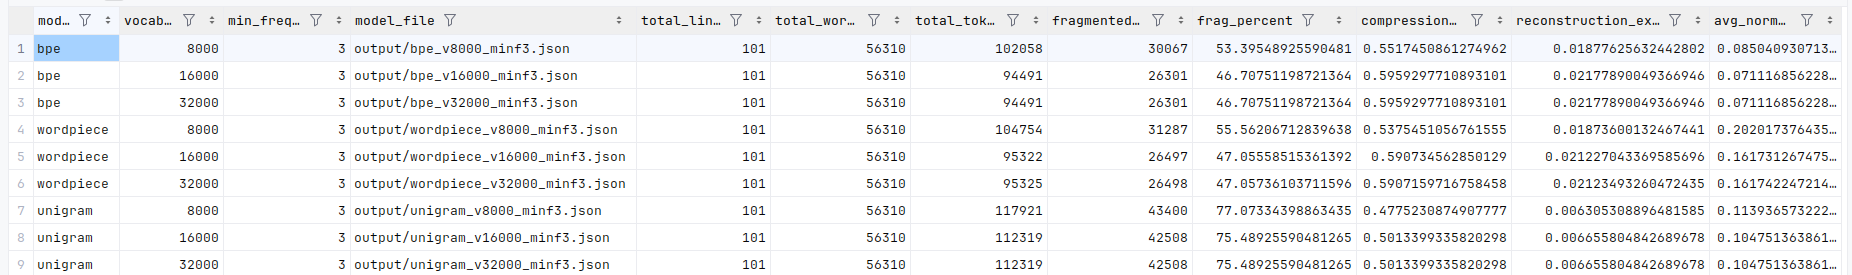
\includegraphics[width=0.9\linewidth]{trainingresults.png}
        			\caption{Пример файла trainingresults.csv}
        			\label{fig:trainingresults}
    			\end{figure}
    			
    			\begin{figure}[h]
        			\centering
        			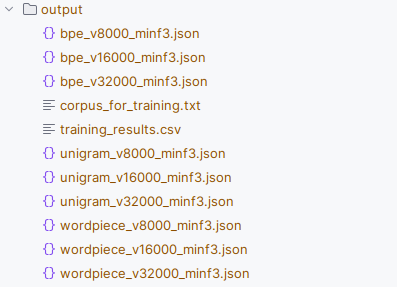
\includegraphics[width=0.9\linewidth]{trainingartefacts.png}
        			\caption{Пример полученных после обучения токенизаторов артефактов}
        			\label{fig:trainingartefacts}
    			\end{figure}
			
		\subsection{Разработка веб-приложения для интерактивного анализа}
		
			На данном этапе мы разрабатываем интерактивное веб-приложение на streamlit для удобного эксперементирования с методами подсловной токенизации.
			
			Оно превращает исследовательский процесс одного из предыдущих этапов (обучение токенизаторов) в удобный инструмент, где можно:
			
			\mystyleitemize{
    				\item загрузить корпус JSONL,
    				\item выбрать тип и параметры токенизатора,
    				\item обучить или применить модель,
    				\item изучить ключевые метрики и распределения,
    				\item экспортировать обученный токенизатор и отчёт.
			}
			
			На рисунке \ref{fig:webapp} можно увидеть вид веб-приложение и часть его функционала. 
			
			\begin{figure}[h]
        			\centering
        			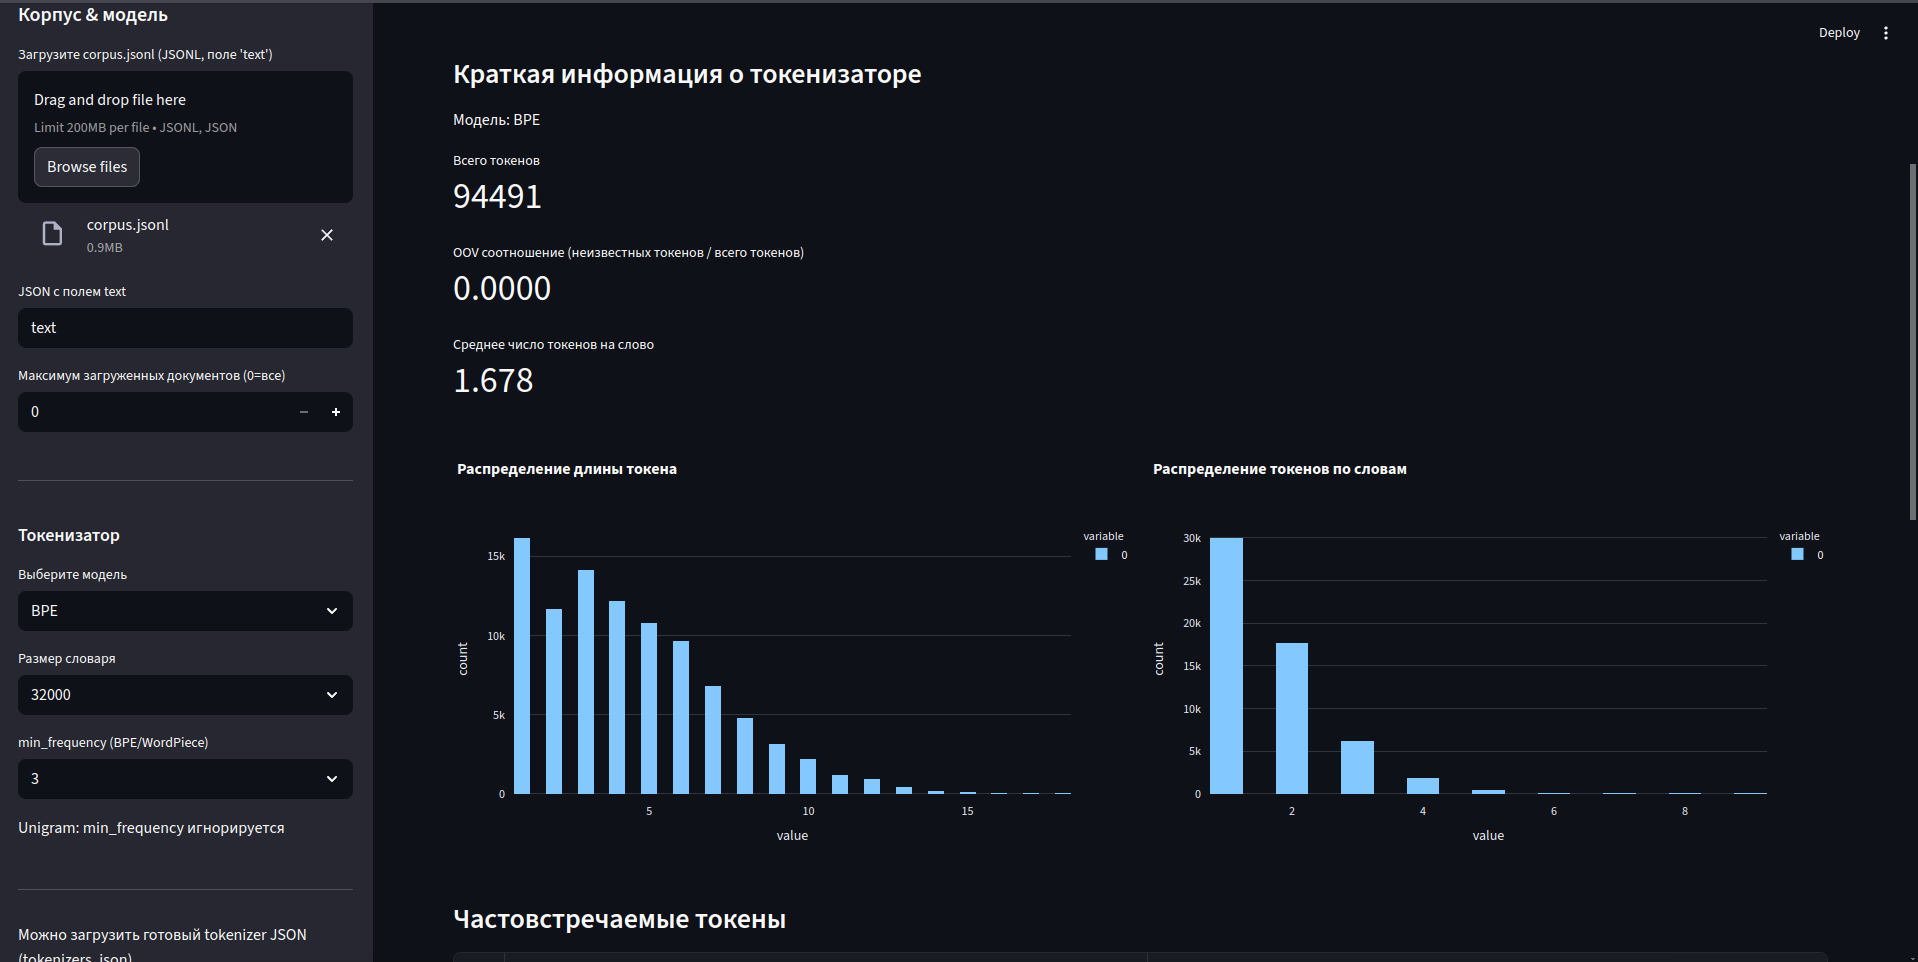
\includegraphics[width=0.9\linewidth]{webapp.png}
        			\caption{Веб-приложение}
        			\label{fig:webapp}
    			\end{figure}
			
		\subsection{Публикация моделей в Hugging Face Hub}
			
			Следующим этапом было публикация обученных токенизаторов на Huggingface. Необходимо выбрать лучшую версию каждого из токенизаторов, выложить их и заполнить карточки.
			
			Кроме того необходимо развернуть веб-приложение на Huggingface spacy.
			
			На рисунке \ref{fig:hf} представлен профиль с развернутым нами веб-приложением и опубликованными токенизаторами. На рисунках \ref{fig:hfbpe1}, \ref{fig:hfbpe2}, \ref{fig:hfbpe3} показан оформленный репозиторий с BPE токенизатором. Остальные токенизаторы оформлены схожим образом, поэтому они не будут показаны.
			
			\begin{figure}[H]
        			\centering
        			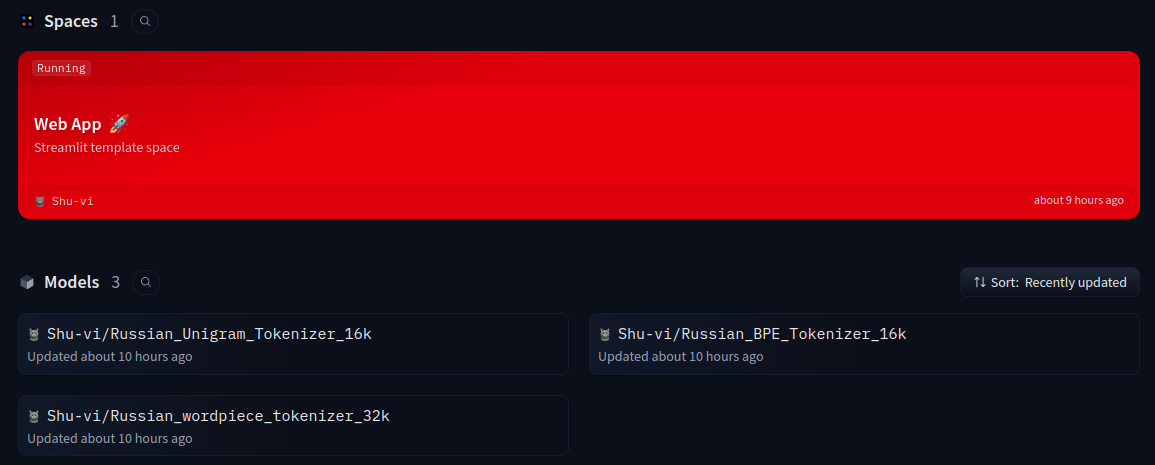
\includegraphics[width=0.9\linewidth]{hf.png}
        			\caption{Профиль на HF с опубликованными моделями и веб-приложением}
        			\label{fig:hf}
    			\end{figure}
    			
    			\begin{figure}[H]
        			\centering
        			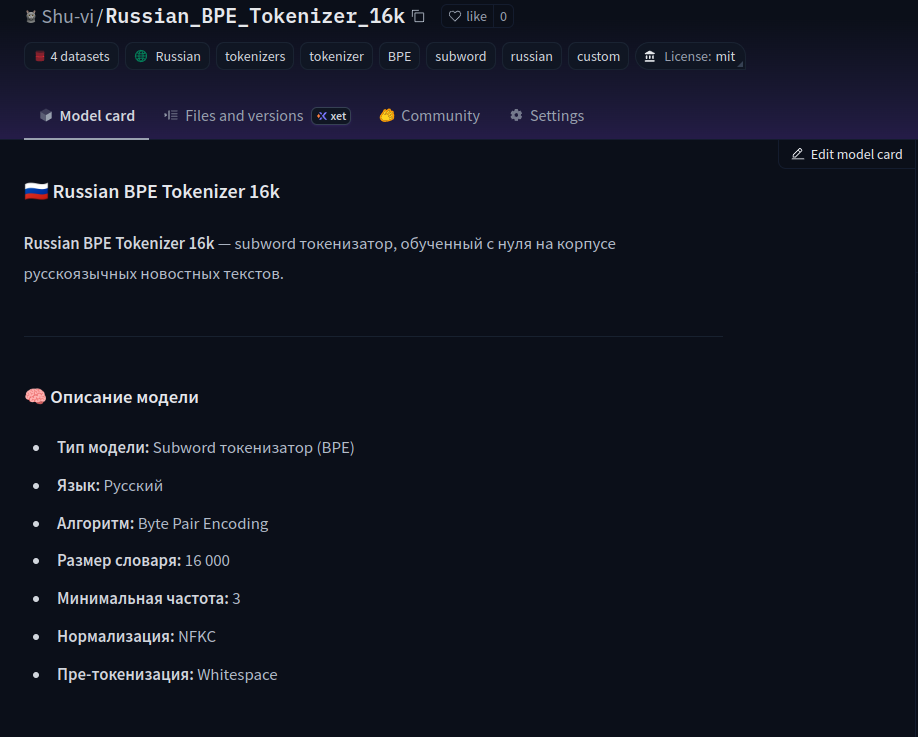
\includegraphics[width=0.9\linewidth]{hfbpe1.png}
        			\caption{Первая часть с оформлением репозитория BPE токенизатора}
        			\label{fig:hfbpe1}
    			\end{figure}
    			
    			\begin{figure}[H]
        			\centering
        			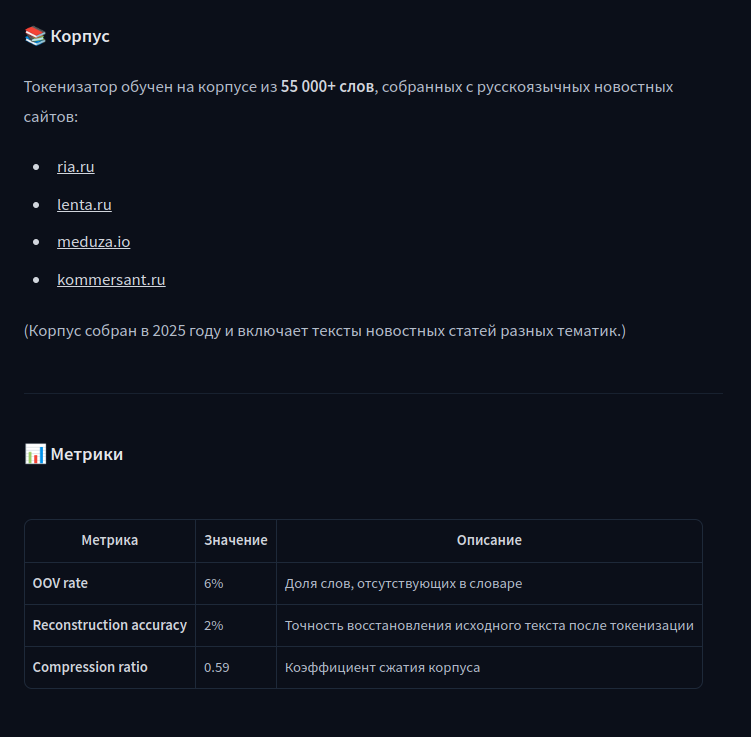
\includegraphics[width=0.9\linewidth]{hfbpe2.png}
        			\caption{Вторая часть с оформлением репозитория BPE токенизатора}
        			\label{fig:hfbpe2}
    			\end{figure}
    			
    			\begin{figure}[H]
        			\centering
        			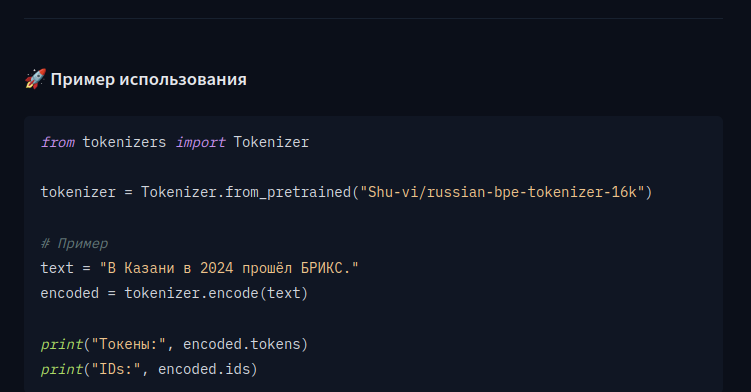
\includegraphics[width=0.9\linewidth]{hfbpe3.png}
        			\caption{Третья часть с оформлением репозитория BPE токенизатора}
        			\label{fig:hfbpe3}
    			\end{figure}
		
	\newpage
	\customsection{ЗАКЛЮЧЕНИЕ}
	
		В ходе выполнения проекта были решены все поставленные задачи и на практике изучен весь конвейер NLP от парсинга текстов и до обучения токенизаторов. Работа позволила получить целостное понимание архитектуры NLP-пайплайна и практический опыт взаимодействия с современными библиотеками для задач NLP.

		Были разработаны:

		\mystyleitemize{
    			\item модуль универсальной предобработки текста, обеспечивающий стандартизацию и очистку корпуса,
    			\item три подсловные модели токенизации -- BPE, WordPiece и Unigram, обученные на едином корпусе и проанализированные по ряду количественных метрик,
    			\item веб-интерфейс Streamlit для интерактивного сравнения токенизаторов, визуализации распределений и экспорта результатов в HTML и CSV.
		}
		
		Реализованные решения опубликованы в открытом доступе:
		
		\mystyleitemize{
    			\item Github-репозиторий проекта: \url{https://github.com/Shu-vi/NLP}
    			\item BPE токенизатор: \url{https://huggingface.co/Shu-vi/Russian_BPE_Tokenizer_16k}
    			\item WordPiece токенизатор: \url{https://huggingface.co/Shu-vi/Russian_wordpiece_tokenizer_32k}
    			\item Unigram токенизатор: \url{https://huggingface.co/Shu-vi/Russian_Unigram_Tokenizer_16k}
    			\item Веб-приложение: \url{https://huggingface.co/spaces/Shu-vi/web-app}
		}
    		
\end{sloppypar}
\end{document}
